\section{问题四：Benchmark 检验与能力演进}
\label{sec:5.5}

问题四把 Benchmark 表现、训练规模与时间变化纳入统一口径，分析开放权重模型能力前沿中规模扩张与非规模因素的贡献，并在算力增速放缓情景下讨论能力演进。需先说明本章结果的数据时点：能力分解基于 $2023.50\to2025.00$ 的历史窗口，情景预测以 $T_0=2025.25$ 为锚点，属条件情景结果；更新数据截止日后需重新预测，相关验收边界集中列于 \ref{sec:7.2}。

\subsection{模型建立}
\label{sec:5.5.1}

\subsubsection{数据口径与样本边界}

主能力指标为 C1/C2 的 \texttt{Average}，由六项 Benchmark 维度等权汇总，量纲为 0--100 分。C2 在 C1 榜单上增加 Epoch 匹配信息，二者属同一批榜单记录。模型类型按榜单标签区分：\texttt{base} 含 pretrained 与 continuously pretrained，\texttt{chat} 含 chat 与 fine-tuned；merges、multimodal 与 other 不纳入两类主回归。C2 发布日用于模型时间轴，C1 提交日用于 C8 月度汇总，两类日期不互换。

本问关注开放权重模型，「权重可获得」与许可证允许的用途是两个字段，许可证未知时保留未知状态。C2 与 C4 先按发布日期和组织匹配，再要求参数量差异小于 $50\%$；训练 token 缺失时由 $D=C/(6N)$ 反解并标记为估算量。C3 混合了不同评测口径，仅作时间趋势敏感性材料，不并入主面板；C5/C6 按可比性分层使用。

\subsubsection{两套实现流程}

本问沉淀了两套实现流程，其来源与状态见表~\ref{tab:q4_flow_status}，二者共同保证方法可对照、结果可追溯。

\begin{table}[H]
\centering\footnotesize
\caption{问题四两套实现流程的来源与状态}
\label{tab:q4_flow_status}
\begin{tabularx}{\textwidth}{@{}p{2.1cm} X X@{}}
\toprule
流程 & 数据、时间轴与产物 & 当前状态 \\
\midrule
主链
& \texttt{q4\_01\_c8\_parse} 至 \texttt{q4\_05\_forecast}；预测接口以 $T_0=2025.25$ 为起点，对应目标日期 2026.25、2027.25；C1/C8 提交日序列截止于 2025-03-13。产物位于 \texttt{src/outputs\_q4/}。
& 现存结果生成于代码与公共接口修订之前，作为历史分析结果使用，更新输入后重跑即可刷新。 \\
补充独立实现
& 入口 \path{src/code_q4/independent/run_q4_independent.py}，配置 \texttt{config\_q4.json}；来源报告记录预测起点 2024-12-31、数据截止 2025-03-13。
& 作为代码实现对照，数值资源链标记 \texttt{DEFERRED\_Q3}，在本仓库独立运行后用于交叉核对。 \\
\bottomrule
\end{tabularx}
\end{table}

\subsubsection{逐任务饱和度与去饱和分}

为降低已接近任务上限的维度对汇总分变化的压缩，先按叶子任务随机基线 $c_j$ 归一化得分：
\[
\hat{s}_{j}=\max\left\{0,\frac{s_j-c_j}{1-c_j}\right\},
\]
再按 C1 提交日构造任务级累计 Top-5 前沿 $F_{t,j}$。去饱和分剔除饱和任务，以起点剩余空间为家族内权重、令六个任务家族等权：
\[
S_{\mathrm{desat},t}=100\sum_j w_j\hat{s}_{j,t},\qquad w_j\propto 1-F_{\mathrm{start},j}.
\]
该分是 \texttt{Average} 的敏感性口径，用于更灵敏地反映尚未饱和任务上的进展。

\begin{figure}[H]
\centering
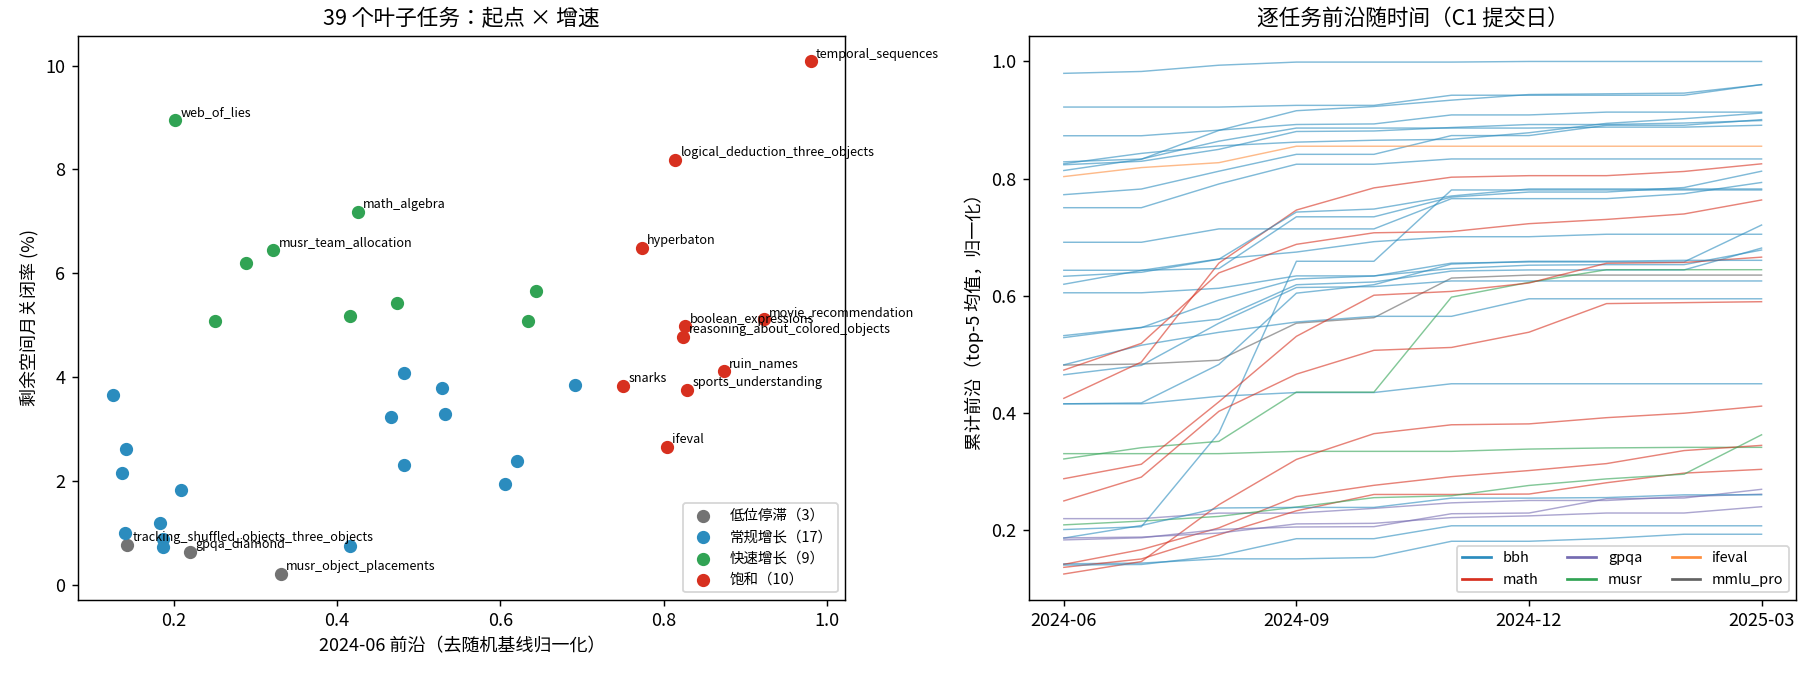
\includegraphics[width=\textwidth]{figs/q4_F9_task_saturation.png}
\caption{C8 叶子任务的饱和度分类}
\label{fig:F9_task_saturation}
\end{figure}

\texttt{P4\_task\_saturation.csv} 含 39 个任务：饱和 10 个、快速增长 9 个、常规增长 17 个、低位停滞 3 个。

\begin{table}[H]
\centering\footnotesize
\caption{能力口径的历史窗口比较（2024-06 至 2025-03；源自 \texttt{T5\_desat\_vs\_average.csv}）}
\label{tab:q4desat}
\begin{tabularx}{\textwidth}{@{}X r r r r@{}}
\toprule
口径 & 起点前沿 & 终点前沿 & 相对变化 & 月斜率 \\
\midrule
C1 \texttt{Average} & 38.52 & 49.89 & 29.53\% & 1.285 \\
C8 全任务重算 & 37.98 & 49.40 & 30.08\% & 1.326 \\
C8 去饱和分 & 26.36 & 39.06 & 48.19\% & 1.536 \\
\bottomrule
\end{tabularx}
\end{table}

去饱和分相对变化明显高于 \texttt{Average}，更充分地显现了未饱和任务上的进步速度。模型级重算与 C1 的一致性中，除 MATH 外五个任务族 Pearson 不低于 $0.989$；MATH 为 $0.801$、MAE $3.497$ 分（\texttt{T5\_c8\_vs\_c1\_check.csv}），该差异原因有待进一步解释。

\begin{figure}[H]
\centering
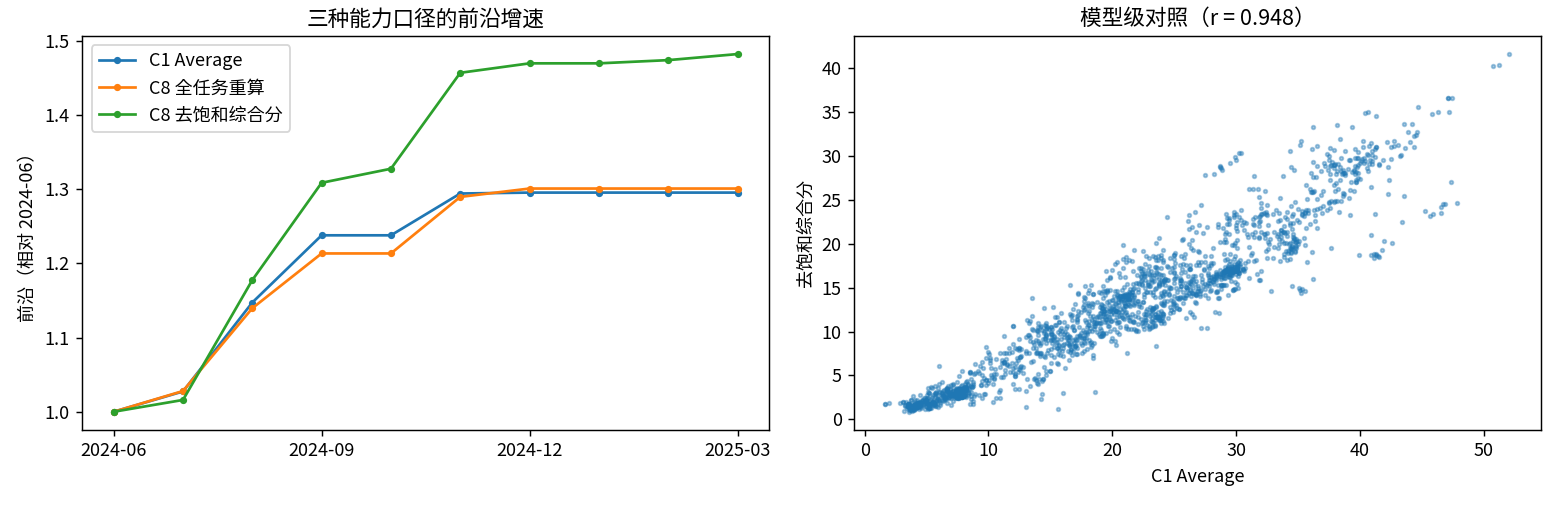
\includegraphics[width=\textwidth]{figs/q4_F10_desat_vs_avg.png}
\caption{去饱和分与 C1 \texttt{Average} 的历史窗口比较}
\label{fig:F10_desat_vs_avg}
\end{figure}

\subsubsection{Loss--Benchmark 桥接}

C6 的损失与 Benchmark 得分按可比性分层后，用有界 S 形函数描述二者关系：
\[
S(L)=lo+\frac{hi-lo}{1+\exp\!\left[k(L-L_0)\right]},\qquad 0\le lo\le hi\le100,\quad k>0,
\]
High 层为同模型、同验证集记录（权重 1），Medium 层验证集不同但近似可比（权重 $0.5$）。\texttt{base|Average} 的参数为 $(lo,hi,k,L_0)=(8.626,21.572,46.119,2.070)$（44 行；C6 含 High 7、Medium 68）。留一比较中 S 形、线性、常数模型 RMSE 为 $8.079$、$8.283$、$9.514$ 分，S 形桥接表现最好。High 层主要约束下界、覆盖底噪区，上升段由 Medium 层决定；面板分解会重估得分映射，C6 固定映射仅作对照。

\begin{figure}[H]
\centering
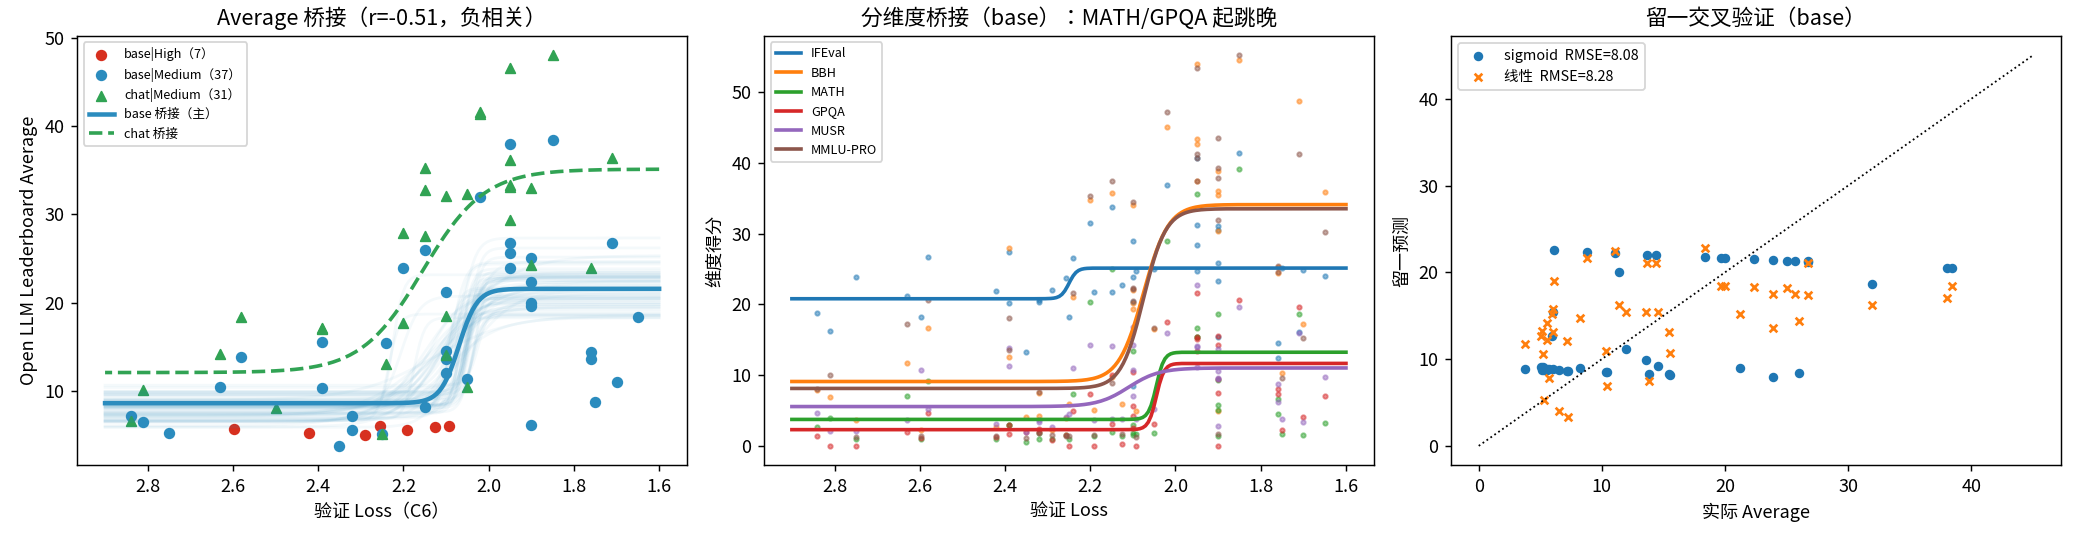
\includegraphics[width=\textwidth]{figs/q4_F11_bridge.png}
\caption{C6 分层 Loss--Benchmark 桥接拟合}
\label{fig:F11_bridge}
\end{figure}

\subsubsection{规模与非规模因素的模型内分解}

每个面板观测把 C2 能力分与 C4 配置连接，再用问题二标度律计算规模状态 $\hat L_i$。主模型 M1b 将非线性映射与时间项相加：
\[
S_i=lo+\frac{amp}{1+\exp\!\left[k(\hat L_i-L_0)\right]}+\tau(t_i-2023)+\varepsilon_i,
\]
$\tau$ 表示控制规模状态后的年度时间关联。对照 M1c 把时间项写入等效年降损 $\delta$：
\[
S_i=lo+\frac{amp}{1+\exp\!\left[k(\hat L_i-\delta(t_i-2023)-L_0\right]}+\varepsilon_i.
\]
另有效率前沿线性模型 M2、分位数回归 M3 与以 $\log_{10}C$ 为解释变量的 OLS。对两端点状态采用双顺序 Shapley 分配\cite{shapley}：
\[
\begin{aligned}
\Delta S_{\mathrm{scale}}={}&\tfrac12\{[f(\hat L_1,t_0)-f(\hat L_0,t_0)]
+[f(\hat L_1,t_1)-f(\hat L_0,t_1)]\},\\
\Delta S_{\mathrm{time}}={}&\tfrac12\{[f(\hat L_0,t_1)-f(\hat L_0,t_0)]
+[f(\hat L_1,t_1)-f(\hat L_1,t_0)]\},\\
\Delta S_{\mathrm{model}}={}&\Delta S_{\mathrm{scale}}+\Delta S_{\mathrm{time}}.
\end{aligned}
\]
技术份额定义为 $\Delta S_{\mathrm{time}}/\Delta S_{\mathrm{model}}$。时间项可能吸收数据质量、后训练、架构与样本构成变化，是控制规模后的条件关联。

\subsection{求解方法}
\label{sec:5.5.2}

主链按 \texttt{q4\_01\_c8\_parse}、\texttt{q4\_02\_saturation}、\texttt{q4\_03\_bridge}、\texttt{q4\_04\_decomp}、\texttt{q4\_05\_forecast} 顺序运行，末尾由 \texttt{q4\_99\_check\_report} 检查接口与报告字段。C8 先解析叶子任务再与榜单匹配；C6 桥接用分层加权最小二乘并以留一法比较形式；C2/C4 按发布日、组织与参数量差异匹配。预测脚本以算力情景更新 $C$，在 $Q=1$、$L_{ctx}=4096$ 的 P2 损失切片上计算规模变化，再锚定到前沿并经 M1b/M1c 映射为分；该计算是 Q2 标度律在 $Q=1$ 切片上的情景推演，不读取 P3 最优配置。

\subsection{结果与分析}
\label{sec:5.5.3}

\subsubsection{历史窗口的增长分解}

base 历史窗口的模型内贡献分解见表~\ref{tab:q4decomp}。主口径 M1b 给出规模贡献 $23.063$、技术贡献 $3.404$，技术占模型解释增量的 $12.86\%$（$90\%$ 区间 $6.07\%$–$21.96\%$）；观测变化为 $24.759$，与模型变化 $26.467$ 相差 $-1.708$。不同模型的技术份额存在明显差异，本文并列报告、不宣称唯一拆分。

\begin{table}[H]
\centering\footnotesize
\caption{base 历史窗口的模型内贡献分解（2023.50$\to$2025.00，$\Delta S_{\rm obs}=24.759$；源自 \texttt{P4\_decomposition.csv}）}
\label{tab:q4decomp}
\begin{tabularx}{\textwidth}{@{}l X r r r r r@{}}
\toprule
方法 & 规模项 & 时间项 & 模型变化 & 时间项占比 & 90\% 区间 \\
\midrule
M1b & 23.063 & 3.404 & 26.467 & 12.86\% & 6.07\%--21.96\% \\
M1c & 20.115 & 6.037 & 26.153 & 23.09\% & 4.17\%--45.49\% \\
M2 & 7.358 & 6.186 & 13.544 & 45.67\% & 8.68\%--59.88\% \\
M3 ($q=0.75$) & 7.398 & 4.445 & 11.844 & 37.53\% & $-47.38\%$--58.24\% \\
OLS & 7.722 & 3.235 & 10.957 & 29.53\% & 10.94\%--46.13\% \\
\bottomrule
\end{tabularx}
\end{table}

\begin{figure}[H]
\centering
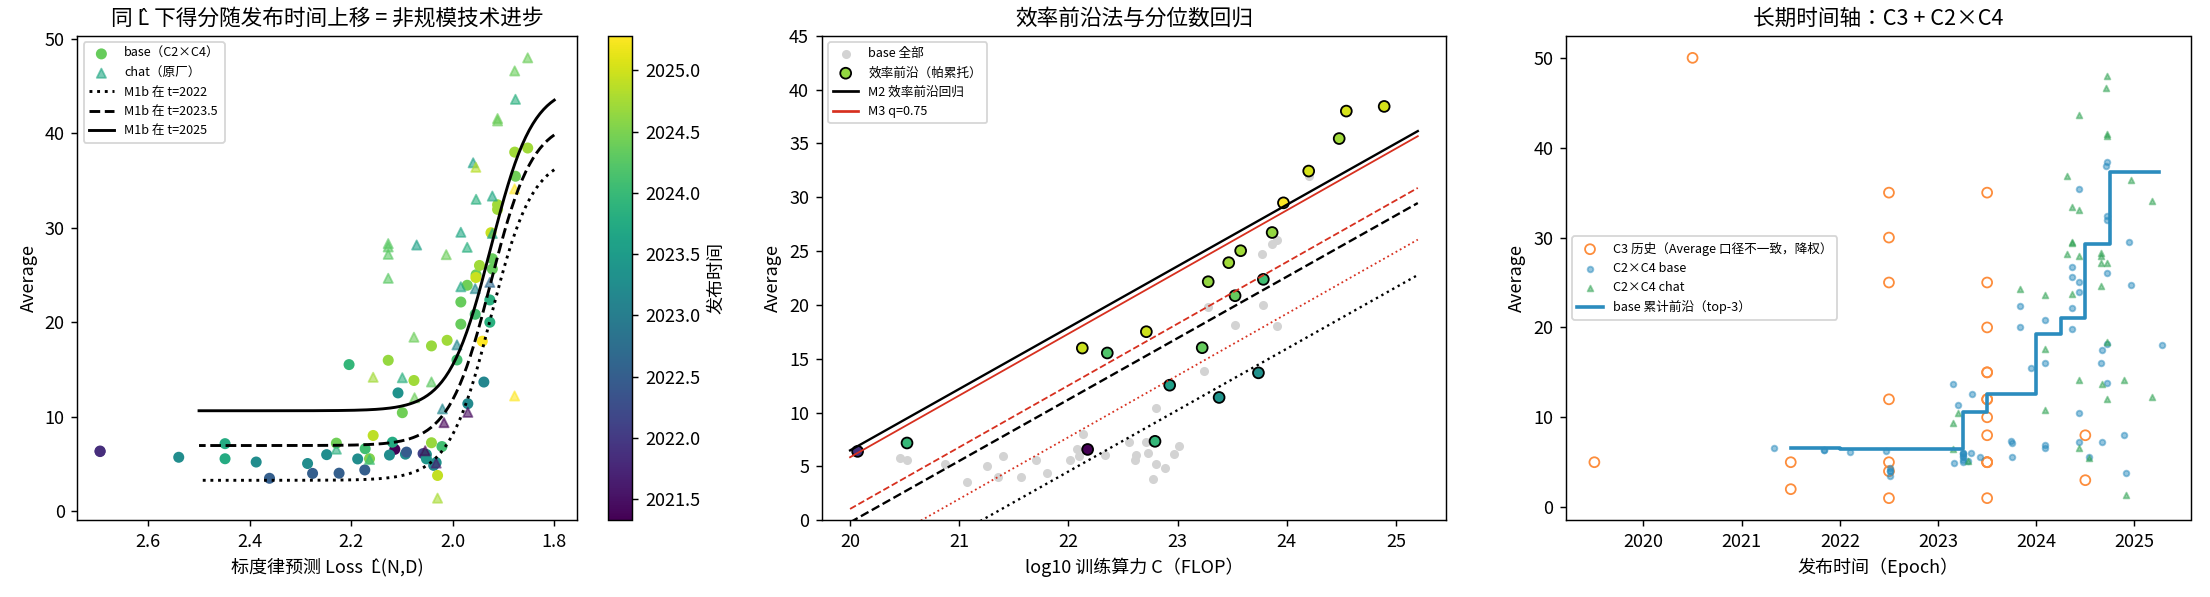
\includegraphics[width=\textwidth]{figs/q4_F12_decomp_panel.png}
\caption{面板中的规模状态、能力分数与时间}
\label{fig:F12_decomp_panel}
\end{figure}

M1b、M1c 的面板 $R^2$ 为 $0.870$、$0.868$，OLS 为 $0.660$（\texttt{T7\_decomp\_fit\_quality.csv}），结构模型对能力分具有良好的解释力。

\begin{figure}[H]
\centering
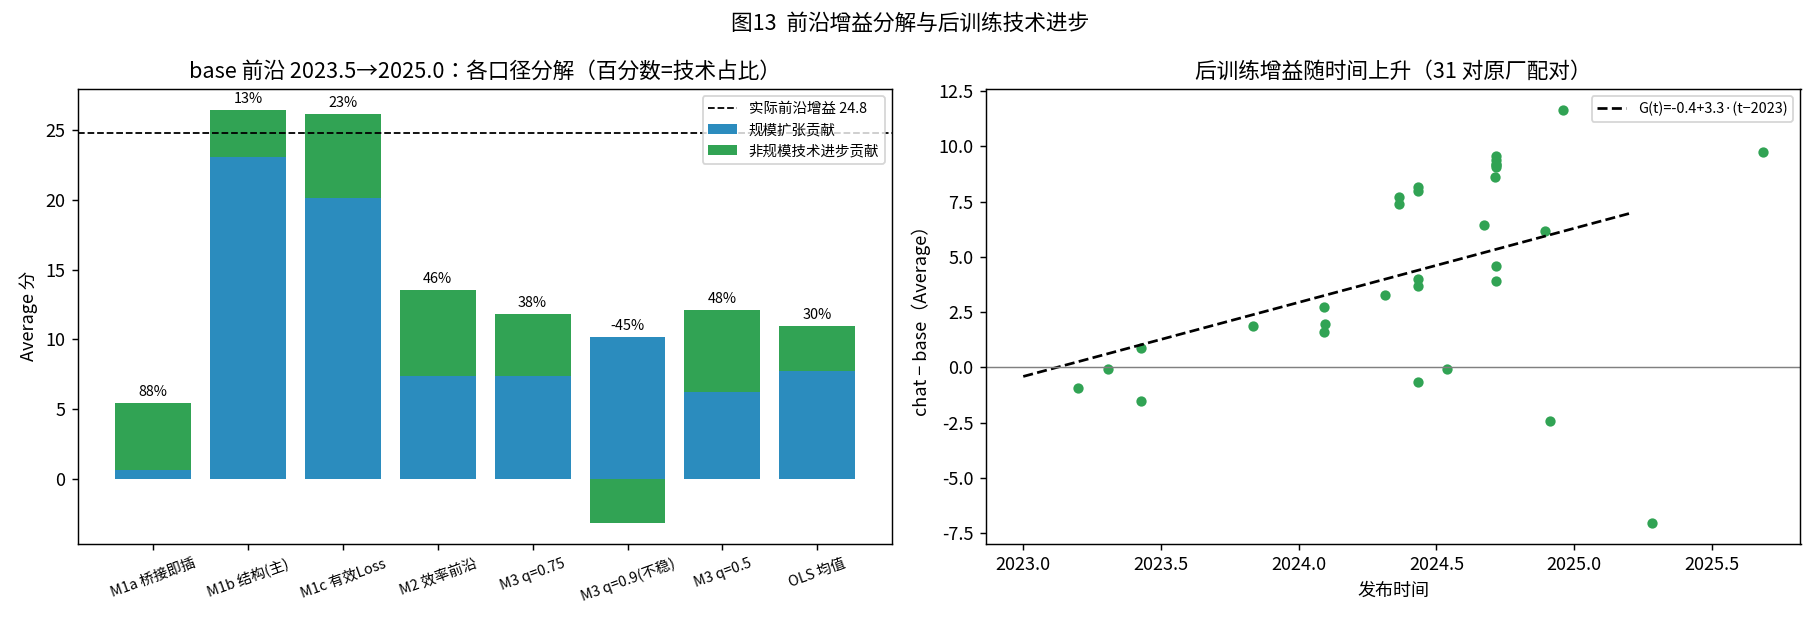
\includegraphics[width=\textwidth]{figs/q4_F13_decomp_bars.png}
\caption{不同模型与窗口下的规模项与时间项}
\label{fig:F13_decomp_bars}
\end{figure}

C3 敏感性显示，仅用 C2$\times$C4 base 样本时算力等效速率为 $0.781$ dex/年，加入 C3（权重 $0.2$、$1.0$）时为 $0.499$、$0.205$ dex/年，时间趋势对历史口径较敏感，故 C3 仅作对照（\texttt{T7\_c3\_sensitivity.csv}）。换用 $2024\to2025$、$2024.5\to2025.25$ 窗口时 M1b 技术占比为 $7.06\%$、$8.18\%$，「规模扩张为主」的定性结论在各窗口下保持稳定。

\subsubsection{算力情景与回测}

锚点 base 得分为 $37.302$、chat 为 $46.057$。表~\ref{tab:q4fc} 给出三种算力增速下的 base 条件分数：算力增速由 $0.60$ 降至 $0.15$ dex/年时，24 个月 base 中位数由 $46.19$ 降至 $44.11$，而时间项占模型变化的比例由 $54.94\%$ 升至 $76.70\%$——算力增长越慢，技术进步越成为能力增量的主体。

\begin{table}[H]
\centering\footnotesize
\caption{按算力增速的 base 条件分数情景（中位数及 $5\%$--$95\%$ 分位；起点 $T_0=2025.25$；源自 \texttt{P4\_frontier\_forecast.csv}）}
\label{tab:q4fc}
\begin{tabularx}{\textwidth}{@{}l c c c@{}}
\toprule
算力增速 & base 12 个月 & base 24 个月 & 24 个月时间项占比 \\
\midrule
0.60 dex/年 & 43.07 [37.35, 52.83] & 46.19 [37.55, 68.49] & 54.94\% \\
0.30 dex/年 & 41.73 [36.95, 49.66] & 45.25 [37.75, 58.28] & 65.49\% \\
0.15 dex/年 & 41.09 [36.63, 47.59] & 44.11 [37.53, 54.86] & 76.70\% \\
\bottomrule
\end{tabularx}
\end{table}

chat 的 24 个月中位数在后训练线性延续情景为 $61.62[51.79,79.62]$、平台情景为 $54.85[46.43,70.12]$，差异来自情景设定。回测方面，以 2024.5 前的 42 个 base 记录重估并预测 2025.25，M1b 在 $0.60$ dex/年情景下误差为 $-0.784$ 分、采用实际算力增速时为 $+0.212$ 分，均明显优于朴素线性外推（$+2.651$ 分）（\texttt{T8\_backtest.csv}）。

\begin{figure}[H]
\centering
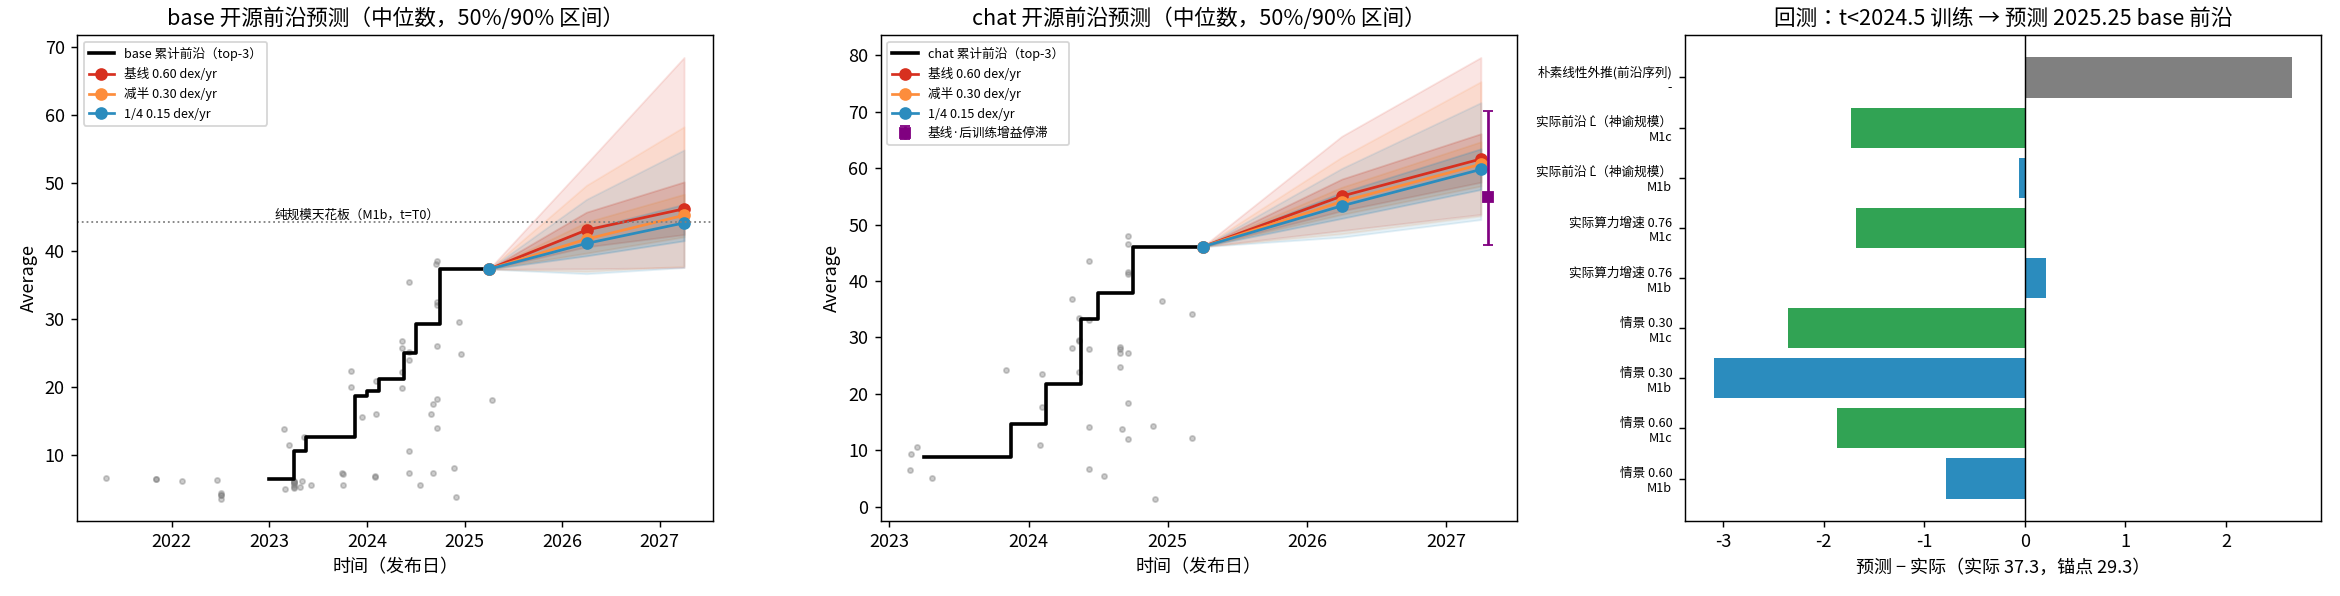
\includegraphics[width=\textwidth]{figs/q4_F14_forecast.png}
\caption{算力情景分数模拟与回测记录}
\label{fig:F14_forecast}
\end{figure}

上述区间混合了 P2 参数抽样、分解模型簇抽样、后训练增益与面板残差，C6 桥接的跨域迁移误差尚未单独传播；个别低算力情景的下界低于锚点，与累计前沿不下降的定义存在张力，重跑时需先修复单调性。这些条件性质已集中列入 \ref{sec:7.2}，不影响「规模扩张为主、技术进步约占一成到两成、算力放缓时技术贡献上升」这一核心结论。
